\setcounter{page}{2}
\section*{Цель работы.}
Разработать программу, реализующую отображение полиномиальной кривой с помощью кубических сплайнов.

\section*{Задание.}
Реализовать интерактивное приложение, отображающее заданные полиномиальные кривые. При этом для кривых, состоящих из нескольких сегментов, должно быть обеспечено свойство непрерывной кривизны. Программа должна позволять пользователю: интерактивно менять положение контрольных точек.

Вариант 11. NURB-сплайн (n = 6, k = 3) с равномерным узловым вектором и изменяемыми весами точек.
В отчете д.б. представлена реализуемая в программе формула, описан алгоритм построения и показаны основные характеристики кривой


\section*{Основные теоретические положения.}
Сплайны - это гладкие (имеющие несколько непрерывных производных) кусочно-полиномиальные функции, которые могут быть использованы для представления функций, заданных большим количеством значений и для которых неприменима аппроксимация одним полиномом. Так как сплайны гладки, экономичны и легки в работе, они используются при построении произвольных функций для:
\begin{itemize}
    \item моделирования кривых;
    \item аппроксимации данных с помощью кривых;
    \item выполнения функциональных аппроксимаций;
    \item решения функциональных уравнений.
\end{itemize}

Неоднородный рациональный B-сплайн, NURBS (Non-uniform rational B-spline) - математическая форма, применяемая в компьютерной графике для генерации и представления кривых и поверхностей. В общем случае В-сплайн состоит из нескольких сплайновых сегментов, каждый из которых определен как набор управляющих точек. Поэтому коэффициенты многочлена будут зависеть только от управляющих точек на рассматриваемом сегменте кривой. Этот эффект называется локальным управлением, поскольку перемещение управляющей точки будет влиять не на все сегменты кривой.

Аналитически B-сплайн описывается тремя объектами: набором из $n+1$ контрольной точки
\(\mathbf{P}_{i}  \; (0\leq i \leq n)\), узловым вектором $U$, состоящим из $m + 1$ узла  \(0 = u_0 \leq
u_1 \leq u_2 \dots \leq u_{m-1} \leq u_m = 1\) и степенью $p$ удовлетворяющей условию \(m=n+p+1\).
Уравнение имеет вид:
\begin{displaymath}
    \mathbf{C} (u) = \sum_{i=0}^{n} N_{i,p}(u)\mathbf{P}_i
\end{displaymath}
где \(N_{i,p}(u)\) $i$-тая базисная функция B-сплайна степени $p$, определяемая рекурсивно:
\begin{displaymath}
    N_{i,0}(u) = \begin{cases}
                     1, & \mbox{if } u \in [u_i,u_{i+1})\\
                     0, & \mbox{otherwise}
    \end{cases}
\end{displaymath}
\begin{displaymath}
    N_{i,p}(u) = \frac{u-u_i}{u_{i+p}-u_i}N_{i,p-1}(u)+\frac{u_{i+p+1}-u}{u_{i+p+1}-u_{i+p}}N_{i+1,p-1}(u)
\end{displaymath}
NURBS кривая добавляет веса \(w_i \geq 0\) к контрольной точке \(\mathbf{P}_{i}\).
Получаем уравнение:
\begin{displaymath}
    \mathbf{C} (u) = \frac{1}{\sum_{i=0}^{n}N_{i,p}(u) w_i}\sum_{i=0}^{n} N_{i,p}(u) w_i \mathbf{P}_i
    = \sum_{i=0}^{n}R_{i,p}(u)\mathbf{P}_{i}
\end{displaymath}
где \(R_{i,p}(u) = N_{i,p}(u) w_i/\sum_{i=0}^{n}N_{i,p}(u) w_i\), $i$ пробегает по базисным функциям.
Пример NURBS кривой приведен на рисунке 1.
\begin{figure}[H]
    \centering
    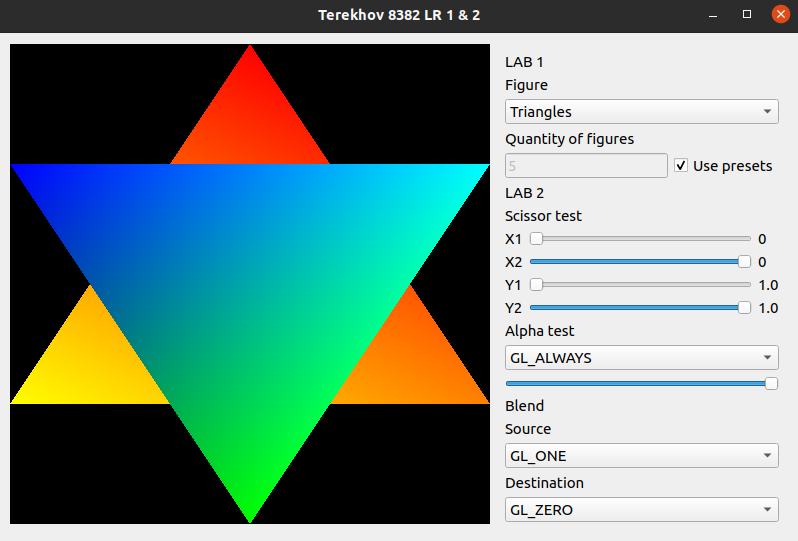
\includegraphics[width=10cm]{1}
    \caption*{Рисунок 1 -- Пример NURBS кривой}
    \label{fig:1}
\end{figure}

\section*{Выполнение работы.}
Для выполнения работы был выбран язык Python 3.8 с библиотеками PyQt5 и PyOpenGL.
Для их установки необходимо воспользоваться командами:\\
\texttt{pip install pyqt5 PyOpenGL PyOpenGL\_accelerate}

Запуск программы:\\
\texttt{python3 main.py}

Для реализации построения NURBS 3 степени по 6 точкам, был описан класс \texttt{NURBSpline3deg6points}.
\begin{lstlisting}[label={lst:1}]
class NURBSpline3deg6points(BSpline):
    def __init__(self, points):
        assert len(points) == 6
        super().__init__(3, [i / 9 for i in range(10)], [point.get_weight() for point in points],
                         [point.get_coordinates().values() for point in points])
    ...
    def _nurbs_curve(self, u):
        return np.sum([self._nurbs_basis_function(i, u) * self._control_points[i] for i in range(len(self._weights))],
                      axis=0)

    def get_nurbs_curve_points(self):
        x = np.arange(0, 1, step=0.01)
        return [self._nurbs_curve(i) for i in x][1:]
    ...
\end{lstlisting}

В функции \verb get_nurbs_curve_points  перебираются значения параметра $u$ (см. теор. положения) и строится кривая по формулам выше.

Вычисление значений базисных функций B-сплайна описано в классе \verb BSpline.
Так как базисная функция рекурсивна, её значения на тройках аргументов будет разумно кэшировать:
\begin{lstlisting}
    if (i, p, u) in self._cache:
        return self._cache.get((i, p, u))
\end{lstlisting}

С полным исходным кодом программы можно ознакомиться по ссылке:
https://github.com/snchz29/CG/tree/lab\_3.

Интерфейс программы состоит из графической зоны и панели с информацией (см. рис. 2).
\begin{figure}[H]
    \centering
    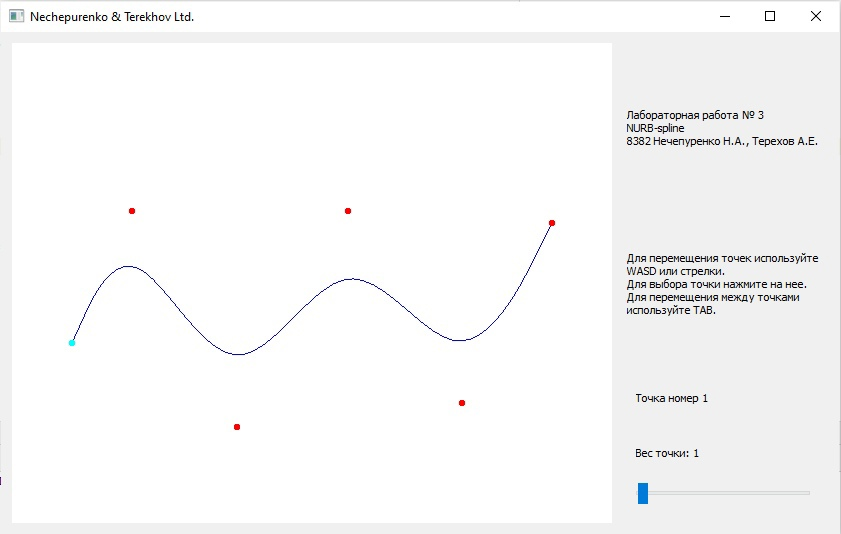
\includegraphics[width=15cm]{2}
    \caption*{Рисунок 2 -- Интерфейс программы}
    \label{fig:2}
\end{figure}

При нулевом значении веса $i$-той точки, она перестает влиять на кривую (см. рис. 3).
\begin{figure}[H]
    \centering
    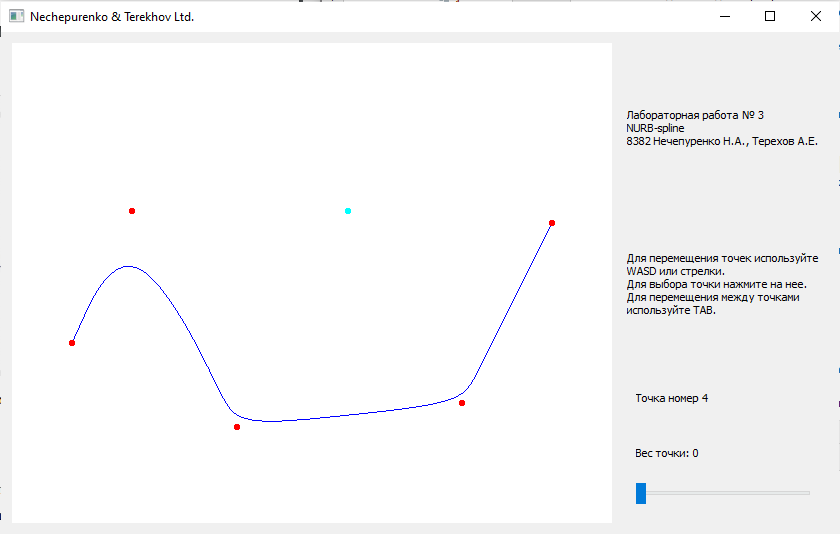
\includegraphics[width=15cm]{3}
    \caption*{Рисунок 3 -- Наличие точки с нулевым весом}
    \label{fig:3}
\end{figure}

Передвинем немного точки и увеличим вес одной третьей точки (см. рис. 4).
\begin{figure}[H]
    \centering
    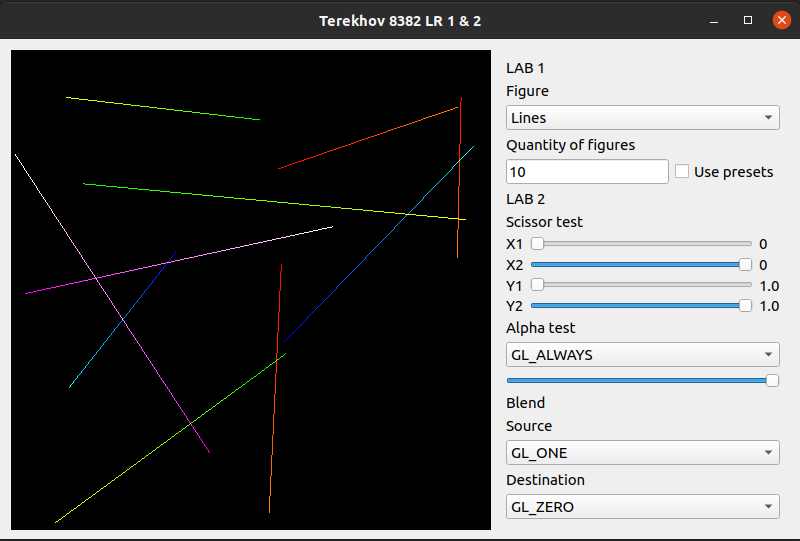
\includegraphics[width=15cm]{4}
    \caption*{Рисунок 4 -- Наличие точки с большим весом}
    \label{fig:4}
\end{figure}

Участок кривой, управляемый данной точкой становится более крутым.

\section*{Выводы.}
В ходе выполнения лабораторной работы была реализована программа, позволяющая визуализировать NURBS кривую.
Были получены навыки построения базисных функций кубических сплайнов, с последующим их использованием.
Интерфейс реализованной программы позволяет передвигать контрольные точки, а также изменять их веса.